%%%%%%%%%%%%%%%%%%%%%%%%%%%%%%%%%%%%%%%%%%%%%%%%%%%%%%%%%%%%%%%%%%%%%%%%%%%%%%%%
%2345678901234567890123456789012345678901234567890123456789012345678901234567890
%        1         2         3         4         5         6         7         8

\documentclass[letterpaper, 10 pt, conference]{ieeeconf}

    \usepackage{graphicx}
    \usepackage[backend=biber]{biblatex}
    \usepackage{pgfplots}
    \documentclass{scrreprt}
    \makeatletter
    \usepackage{color}
    \definecolor{lightgray}{rgb}{0.95, 0.95, 0.95}
    \definecolor{darkgray}{rgb}{0.4, 0.4, 0.4}
    %\definecolor{purple}{rgb}{0.65, 0.12, 0.82}
    \definecolor{editorGray}{rgb}{0.95, 0.95, 0.95}
    \definecolor{editorOcher}{rgb}{1, 0.5, 0} % #FF7F00 -> rgb(239, 169, 0)
    \definecolor{editorGreen}{rgb}{0, 0.5, 0} % #007C00 -> rgb(0, 124, 0)
    \definecolor{orange}{rgb}{1,0.45,0.13}		
    \definecolor{olive}{rgb}{0.17,0.59,0.20}
    \definecolor{brown}{rgb}{0.69,0.31,0.31}
    \definecolor{purple}{rgb}{0.38,0.18,0.81}
    \definecolor{lightblue}{rgb}{0.1,0.57,0.7}
    \definecolor{lightred}{rgb}{1,0.4,0.5}
    \usepackage{upquote}
    \usepackage{listings}
    % CSS
    \lstdefinelanguage{CSS}{
      keywords={color,background-image:,margin,padding,font,weight,display,position,top,left,right,bottom,list,style,border,size,white,space,min,width, transition:, transform:, transition-property, transition-duration, transition-timing-function},	
      sensitive=true,
      morecomment=[l]{//},
      morecomment=[s]{/*}{*/},
      morestring=[b]',
      morestring=[b]",
      alsoletter={:},
      alsodigit={-}
    }
    
    % JavaScript
    \lstdefinelanguage{JavaScript}{
      morekeywords={typeof, new, true, false, catch, function, return, null, catch, switch, var, if, in, while, do, else, case, break},
      morecomment=[s]{/*}{*/},
      morecomment=[l]//,
      morestring=[b]",
      morestring=[b]'
    }
    
    \lstdefinelanguage{HTML5}{
      language=html,
      sensitive=true,	
      alsoletter={<>=-},	
      morecomment=[s]{<!-}{-->},
      tag=[s],
      otherkeywords={
      % General
      >,
      % Standard tags
        <!DOCTYPE,
      </html, <html, <head, <title, </title, <style, </style, <link, </head, <meta, />,
        % body
        </body, <body,
        % Divs
        </div, <div, </div>, 
        % Paragraphs
        </p, <p, </p>,
        % scripts
        </script, <script,
      % More tags...
      <canvas, /canvas>, <svg, <rect, <animateTransform, </rect>, </svg>, <video, <source, <iframe, </iframe>, </video>, <image, </image>, <header, </header, <article, </article
      },
      ndkeywords={
      % General
      =,
      % HTML attributes
      charset=, src=, id=, width=, height=, style=, type=, rel=, href=,
      % SVG attributes
      fill=, attributeName=, begin=, dur=, from=, to=, poster=, controls=, x=, y=, repeatCount=, xlink:href=,
      % properties
      margin:, padding:, background-image:, border:, top:, left:, position:, width:, height:, margin-top:, margin-bottom:, font-size:, line-height:,
        % CSS3 properties
      transform:, -moz-transform:, -webkit-transform:,
      animation:, -webkit-animation:,
      transition:,  transition-duration:, transition-property:, transition-timing-function:,
      }
    }
    
    \lstdefinestyle{htmlcssjs} {%
      % General design
    %  backgroundcolor=\color{editorGray},
      basicstyle={\footnotesize\ttfamily},   
      frame=b,
      % line-numbers
      xleftmargin={0.75cm},
      numbers=left,
      stepnumber=1,
      firstnumber=1,
      numberfirstline=true,	
      % Code design
      identifierstyle=\color{black},
      keywordstyle=\color{blue}\bfseries,
      ndkeywordstyle=\color{editorGreen}\bfseries,
      stringstyle=\color{editorOcher}\ttfamily,
      commentstyle=\color{brown}\ttfamily,
      % Code
      language=HTML5,
      alsolanguage=JavaScript,
      alsodigit={.:;},	
      tabsize=2,
      showtabs=false,
      showspaces=false,
      showstringspaces=false,
      extendedchars=true,
      breaklines=true,
      % German umlauts
      literate=%
      {Ö}{{\"O}}1
      {Ä}{{\"A}}1
      {Ü}{{\"U}}1
      {ß}{{\ss}}1
      {ü}{{\"u}}1
      {ä}{{\"a}}1
      {ö}{{\"o}}1
    }
    %
    \lstdefinestyle{py} {%
    language=python,
    literate=%
    *{0}{{{\color{lightred}0}}}1
    {1}{{{\color{lightred}1}}}1
    {2}{{{\color{lightred}2}}}1
    {3}{{{\color{lightred}3}}}1
    {4}{{{\color{lightred}4}}}1
    {5}{{{\color{lightred}5}}}1
    {6}{{{\color{lightred}6}}}1
    {7}{{{\color{lightred}7}}}1
    {8}{{{\color{lightred}8}}}1
    {9}{{{\color{lightred}9}}}1,
    basicstyle=\footnotesize\ttfamily, % Standardschrift
    numbers=left,               % Ort der Zeilennummern
    %numberstyle=\tiny,          % Stil der Zeilennummern
    %stepnumber=2,               % Abstand zwischen den Zeilennummern
    numbersep=5pt,              % Abstand der Nummern zum Text
    tabsize=4,                  % Groesse von Tabs
    extendedchars=true,         %
    breaklines=true,            % Zeilen werden Umgebrochen
    keywordstyle=\color{blue}\bfseries,
    frame=b,
    commentstyle=\color{brown}\itshape,
    stringstyle=\color{editorOcher}\ttfamily, % Farbe der String
    showspaces=false,           % Leerzeichen anzeigen ?
    showtabs=false,             % Tabs anzeigen ?
    xleftmargin=17pt,
    framexleftmargin=17pt,
    framexrightmargin=5pt,
    framexbottommargin=4pt,
    %backgroundcolor=\color{lightgray},
    showstringspaces=false,      % Leerzeichen in Strings anzeigen ?
    }%
    %
    \makeatother
    
    \IEEEoverridecommandlockouts                              % This command is only needed if 
       % you want to use the \thanks command
    
    \overrideIEEEmargins                                      % Needed to meet printer requirements.
    
    % See the \addtolength command later in the file to balance the column lengths
    % on the last page of the document
    
    % The following packages can be found on http:\\www.ctan.org
    %\usepackage{graphics} % for pdf, bitmapped graphics files
    %\usepackage{epsfig} % for postscript graphics files
    %\usepackage{mathptmx} % assumes new font selection scheme installed
    %\usepackage{times} % assumes new font selection scheme installed
    %\usepackage{amsmath} % assumes amsmath package installed
    %\usepackage{amssymb}  % assumes amsmath package installed
    
    \title{\LARGE \bf
    Visualize Force closure for 2D Robotic Grasp
    }
    
    
    \author{Ghoshan Jaganathamani$^{1}$% <-this % stops a space
    \thanks{*This work was not supported by any organization}% <-this % stops a space
    \thanks{$^{1}$Ghoshan Jaganathamani is a 3rd year Computer Engineering Student,
            Hong Kong University of Science and Technology, Hong Kong
            {\tt\small github.com/ghoshanjega}}%
    }
    
    \addbibresource{springer.bib}
    
    \begin{document}
    
    
    
    \maketitle
    \thispagestyle{empty}
    \pagestyle{empty}
    
    
    %%%%%%%%%%%%%%%%%%%%%%%%%%%%%%%%%%%%%%%%%%%%%%%%%%%%%%%%%%%%%%%%%%%%%%%%%%%%%%%%
    \begin{abstract}
    
    —This paper presents an approach to robotic grasping analysis. It shows how to check for feasibility of the grasp considered and then measure the quality of the grasp.
    
    \end{abstract}
    
    
    %%%%%%%%%%%%%%%%%%%%%%%%%%%%%%%%%%%%%%%%%%%%%%%%%%%%%%%%%%%%%%%%%%%%%%%%%%%%%%%%
    \section{INTRODUCTION}
    
        Grasping and manipulation with complex grippers, such as multifingered and/or under actuated hands, is an active research area in robotics. The goal of a grasp is to achieve a desired object constraint in the presence of external disturbances (including the object’s own weight). Dexterous manipulation involves changing the object’s position with respect to the hand without any external support.
    
    \section{RELATED WORK}
    In this paper our focus is the interaction between the robot and its environment. The desired behavior of the robot
    hand or end-effector, the contact interface between
    the robot and objects. The focus is on manipulation. We will assume
    that the manipulator, objects, and obstacles in the environment are rigid. The key aspects of robotics grasping are that,
    \subsection{Disturbance resistance}
    
     A grasp can resist disturbances in any direction when object immobility is ensured, either by finger positions (form closure) or, up to a certain magnitude, by the forces applied by the fingers (force closure). Main problem: determination of contact points on the object boundary.
    
    \subsection{Dexterity}
    
    A grasp is dexterous if the hand can move the object in a compatible way with the task to be performed. When there are no task specifications, a grasp is considered dexterous if the hand is able to move the object in any direction. Main problem: determination of hand configuration.
    
    \subsection{Equilibrium}
    
    A grasp is in equilibrium when the resultant of forces and torques applied on the object (by the fingers and external disturbances) is null. Main problem: determination and control of the proper contact forces.
    
    \subsection{Stability}
    
    A grasp is stable if any error in the object position caused by a disturbance disappears in time after the disturbance vanishes. Main problem: control of restitution forces when the grasp is moved away from equilibrium.
    
    
    
    
    \section{UI}
    The user of the program is greeted with a simple website built using HTML and JavaScript for maximum portability. By using JavaScript the program can be embedded in websites, allowing if to be highly portable. The sketching library used in this case is {\tt two.js}, a simple 2D sketching suite. The user for example can input a set of instructions in the respective boxes in the following manner.
    
    {\tt\small alpha : 0.7,\\ number of sides : 5,\\ vertices: 24 45 102 30 150 60 155 117 30 120}
    
    
    \begin{figure}[h]
    \caption{Shows the user interface}
    \centering
    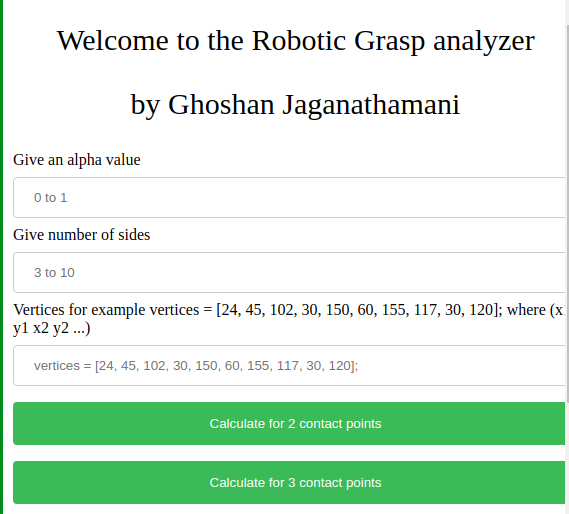
\includegraphics[width=7cm]{ui.png}
    \end{figure}
    
    \section{2 CONTACT POINT GRASP}
    The user inputs the friction coefficient (alpha) and the number of sides the polygon should be. Then the user needs to input the x,y vertices coordinates of the polygon. After the polygon is constructed(make sure the polygon is not self intersecting), the polygon will be displayed on the screen. 
    
    After the polygon sides are constructed, each side has evenly spaced 9 points. So if it is a 5  sided polygon, there will be totally 45 ( 9 * 5 ) points. Then a point is chosen in random using the {\tt\small Math.rand()} function. The selected point {\tt\small p1} will then be checked with all the other points for force closure. 
    
    The wrench matrix is constructed from the 2 contact points. The coefficient of friction produces the alpha angle. The two contact points yield force close if 
    
    \begin{itemize}
        \item rank F = n
        \item there exists a solution to linear optimization to find the minimum for the given wrench matrix.
    \end{itemize}
    
    If the given two contact points yield force closure, a line is drawn between the points indicating compatibility. The points are stored in a  multidimensional array where {\tt points[i] = [x coord, y coord, colour, gradient of line, force closure]}. The results are updated on each calculation step. The user is able to click on the "Calculate for 2 contact points" button repeatedly to find another random point and perform the analysis on the given point.  
    
    
    \begin{figure}[h]
    \caption{Shows 2 instances of 2 contact points calculation}
    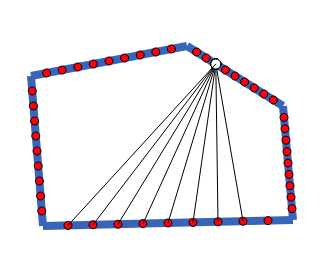
\includegraphics[width=4cm]{2contact1.png}
    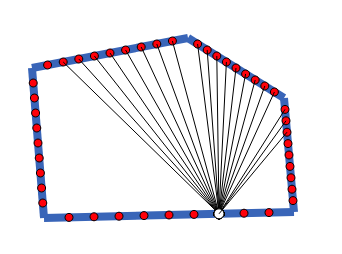
\includegraphics[width=4cm]{2contct2.png}
    \end{figure}
    
    \section{3 CONTACT POINT GRASP}
    Similar to 2 contact point, 3 contact point is calculated with a given random point and 2 compatible points are chosen. This is done recursively when 2 contact points are compatible.
    
    \begin{figure}[h]
    \caption{Shows 2 instances of 3 contact points calculation}
    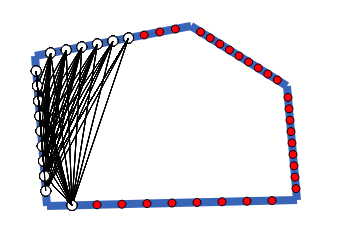
\includegraphics[width=4cm]{3contact1.png}
    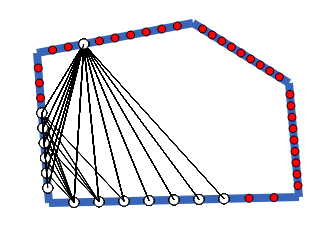
\includegraphics[width=4cm]{3contact2.png}
    \end{figure}
    
    \section{QUALITY of GRASP}
    The quality of the grasp can be measured in many ways. The most accurate way to measure the quality would be to create a 3D Sphere between the contact points 3D wrench space. Since we assume for 2D space, the way to calculate the quality is to find the area of the circle inscribed between the wrench space of the compatible 2 or 3 contact points.  
    \begin{equation}
    Q_{\tiny VOP}=\hbox {Area}(\mathcal{P}) 
    \end{equation}
    
    A plot of for a given point is visualized as follows, where the dependant axis shows all the points that are compare,and independent axis has the the area of the circle inscribed by the wrench matrices.\\
    
    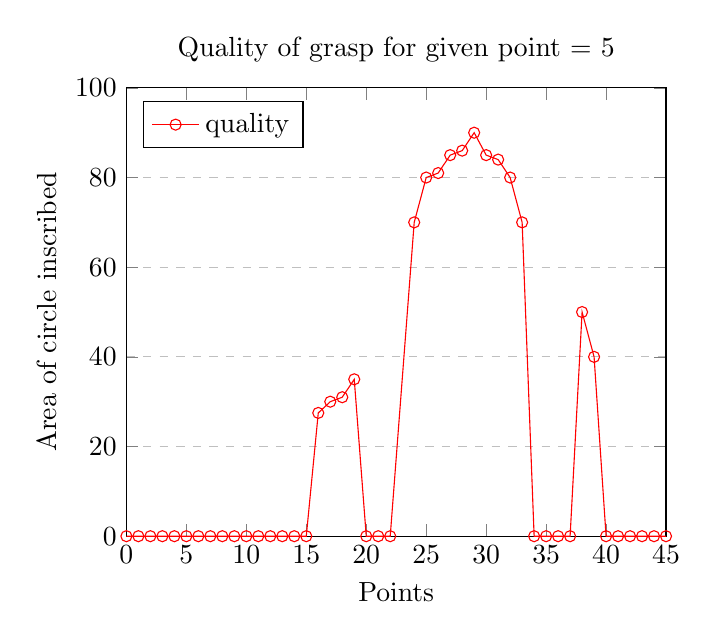
\begin{tikzpicture}
    \begin{axis}[
        title={Quality of grasp for given point = 5},
        xlabel={Points},
        ylabel={Area of circle inscribed},
        xmin=0, xmax=45,
        ymin=0, ymax=100,
        xtick={0,5,10,15,20,25,30,35,40,45},
        ytick={0,20,40,60,80,100},
        legend pos=north west,
        ymajorgrids=true,
        grid style=dashed,
    ]
     
    \addplot[
        color=red,
        mark=o,
        ]
        coordinates {
        (0,0)(1,0)(2,0)(3,0)(4,0)(5,0)(6,0)(7,0)(8,0)(9,0)(10,0)(11,0)(12,0)(13,0)(14,0)(15,0)(16,27.5)(17,30)(18,31)(19,35)(20,0)(21,0)(22,0)(24,70)(25,80)(26,81)(27,85)(28,86)(29,90)(30,85)(31,84)(32,80)(33,70)(34,0)(35,0)(36,0)(37,0)(38,50)(39,40)(40,0)(41,0)(42,0)(43,0)(44,0)(45,0)
        };
        \legend{quality}
     
    \end{axis}
    \end{tikzpicture}
    
    Another quality measure proposed for polyhedral objects and based on a set ICRS is given by the sum of the distances between each one of the   i -th actual contact points   (xi,yi)  and the center of the corresponding independent contact region   (xi0,yi0,zi0) , i.e.\\
    \begin{equation} Q_{\tiny ICR^{\prime \prime }}=\frac{1}{n}\sum \limits _{i=1}^{n}\sqrt{\left( x_i-x_{i0}\right) ^2+\left( y_i-y_{i0}\right) ^2] \end{equation}
    
    \section{CONCLUSION}
    This paper has presented a simple wat to visualize and analyse grasping a 2D polygon with 2 or 3 contact points. The most widely used grasp classifications and closure properties can all be derived from these models under the rigid-body assumption. Linearizing these models leads to metrics and tests that can be computed efficiently using computational linear algebra and linear programming techniques.
    
    Other important research topics within the area of grasping are: grasp synthesis, force distribution, stability, and dexterous manipulation. Grasp synthesis is the problem of choosing the posture of the hand and contact point locations to optimize a grasp quality metric.
    
    The next step would be to prove the stability of the optimal grasp. This could be done using a simulation of external forcesacting on the grasp. To further improve on the grasp, it would be ideal to check the dexterity for better motion planning. Dexterity of the grasp is ability of the hand to move the object in a compatible way with the task to be performed. 
    
    
    \section{REFERENCES}
    
    \begin{itemize}
        \item Grasp quality measures: review and performance, (Article) https://link.springer.com/article/10.1007/s10514-014-9402-
        \item Modern Robotics, (Textbook) http://hades.mech.northwestern.edu/index.php/ModernRobotics
        \item Force Closure grasp, (Article) http://www.centropiaggio.unipi.it/sites/default/files/grasp-IJRR95.pdf
        \item Baker, B.S., Fortune, S., and Grosse, E. 1985. Stable Prehension with a Multifinngered Hand. Proc. IEEE Int. Conf. on Robotics and Automation, pp. 570{575.}
        \item Fearing, R. 1986. Simplied Grasping and Manipulation with Dextrous Robot Hands. IEEE J. Robotics and Automation, vol. 2, no. 4, pp. 188{195.}
        
    \end{itemize}
    
    \onecolumn
    The next file is index.html
    \begin{lstlisting}[style=htmlcssjs]
    
    <!DOCTYPE html>
    <html>
    
    <head>
        <meta charset="utf-8" />
        <meta http-equiv="X-UA-Compatible" content="IE=edge">
        <title>Page Title</title>
        <meta name="viewport" content="width=device-width, initial-scale=1">
        <!-- <script src='js/require.js'></script> -->
        <style>
            #instructions {
                font-family: Times New Roman, Times, serif;
                font-size: 30px;
                text-align: center
            }
    
            body {
                margin: auto;
                border: 3px solid green;
                padding: 10px;
                justify-content: center;
            }
    
            input[type=text],
            select {
                width: 100%;
                padding: 12px 20px;
                margin: 8px 0;
                display: inline-block;
                border: 1px solid #ccc;
                border-radius: 4px;
                box-sizing: border-box;
            }
    
            input[type=submit] {
                width: 100%;
                background-color: #4CAF50;
                color: white;
                padding: 14px 20px;
                margin: 8px 0;
                border: none;
                border-radius: 4px;
                cursor: pointer;
            }
    
            
    
    
            /* input[type=submit]:hover {
                background-color: #45a049;
            } */
        </style>
        <!-- <link rel="stylesheet" type="text/css" media="screen" href="main.css" /> -->
        <script type="text/javascript" src="js/two.js"></script>
        <script type="text/javascript" src="js/SimplexJS.js"></script>
        <!-- <script src="https://cdnjs.cloudflare.com/ajax/libs/p5.js/0.6.1/p5.js"></script> -->
        
    </head>
    
    <body style="align-content: center; width: 100%">
        <p id="instructions">Welcome to the Robotic Grasp analyzer</p>
    
    
        <div style>
            <label for="fname">Give an alpha value</label>
            <input type="text" id="input1" placeholder="0 to 1" />
            <label for="fname">Give number of sides</label>
            <input type="text" id="input2" placeholder="3 to 10" />
            <label for="fname">Vertices for example vertices = [24, 45, 102, 30, 150, 60, 155, 117, 30, 120]; where (x1 y1 x2 y2 ...)</label>
            <input type="text" id="input3" placeholder="vertices = [24, 45, 102, 30, 150, 60, 155, 117, 30, 120];" defaultvalue="24 45 102 30 150 60 155 117 30 120" />
            <!-- <script type="text/javascript" src="js/bundle.js"></script> -->
            <input type="submit" onclick="myJsFunction()" value="Calculate for 2 contact points"></input>
            <input type="submit" onclick="myJsFunction3()" value="Calculate for 3 contact points"></input>
        </div>
        <div style="padding-top: 30px; padding-left: 90px" id="draw-shapes"></div>
        <script type="text/javascript" src="js/2contactpoint.js"></script>
        <script type="text/javascript" src="js/3contactpoint.js"></script>
    
    
    </body>
    
    </html>
    \end{lstlisting}
    
    
    The next file is 2contactpoint.js.
    
    \begin{lstlisting}[style=htmlcssjs]
    
    var alpha, numberofsides, vertices = [];
    var sections = 10;
    var points = [];
    var white = "#FFFFFF";
    var red = "#FF0000";
    
    var elem = document.getElementById('draw-shapes');
    var params = { width: 500, height: 400 };
    var two = new Two(params).appendTo(elem);
    
    function isEmpty(str) {
        return (!str || 0 === str.length);
    }
    
    function myJsFunction() {
        two.clear();
        points = [];
        alpha = document.getElementById('input1').value;
        numberofsides = document.getElementById('input2').value;
        if(!document.getElementById('input3').value)
            vertices = [24, 45, 102, 30, 150, 60, 155, 117, 30, 120];
        else
            vertices = ((document.getElementById('input3').value).split(" "));
        
        console.dir(vertices);
        console.log(alpha,numberofsides,vertices.length,vertices,document.getElementById('input3').value);
        if (drawusershape()) {
            console.log("shape draw called");
        }
    }
    
    
    
    var usershape = [];
    function drawusershape() {
        for (var i = 0, y = 0; i <= vertices.length-3; i += 2, y++) {
            var x1 = vertices[i] * 2;
            var y1 = vertices[i + 1] * 2;
            var x2 = vertices[i + 2] * 2;
            var y2 = vertices[i + 3] * 2;
            console.log(x1, y1, x2, y2);
            var line = two.makeLine(x1, y1, x2, y2);
            line.linewidth = 8;
            line.stroke = '#1C75BC';
            two.update();
            makepoints(x1, y1, x2, y2);
    
        }
    
        var finalline = two.makeLine(vertices[vertices.length - 2] * 2, vertices[vertices.length - 1] * 2, vertices[0] * 2, vertices[1] * 2);
        finalline.linewidth = 8;
        finalline.stroke = '#1C75BC';
        two.update();
        makepoints( vertices[0] * 2, vertices[1] * 2,vertices[vertices.length - 2] * 2, vertices[vertices.length - 1] * 2);
        console.log(points);
        two.update();
        drawpoints();
        runcalc();
        return 1;
    
    }
    
    console.log(red);
    function makepoints(x1, y1, x2, y2) {
        for (var e = 1; e < sections; e++) {
            var gradient = (y2 - y1) / (x2 - x1);
            console.log(y2," - ",y1,") / (",x2," - ",x1," ", -gradient);
            var angle = Math.tan(-1/gradient);
            points.push([x1 + ((x2 - x1) / sections) * e, y1 + ((y2 - y1) / sections) * e, red, - gradient]); //x coord, y coord, colour, gradient
        }
    }
    
    function drawpoints() {
        for (var i = 0; i < points.length; i++) {
            //console.log(points[i],points[i][0],1,points[1][0][0])
            var thispoint = two.makeCircle(points[i][0], points[i][1], 4);
            thispoint.fill = points[i][2];
        }
        two.update();
    }
    
    function updatepoint(thepoint) {
        var thispoint = two.makeCircle(points[thepoint][0], points[thepoint][1], 4);
        thispoint.fill = points[thepoint][2];
        two.update();
    }
    
    function getRandomInt(min, max) {
        return Math.floor(Math.random() * (max - min + 1)) + min;
    }
    
    function runcalc() {
        var selectedpoint = getRandomInt(0, points.length-1);
        console.log(selectedpoint);
        points[selectedpoint][2] = "#9932CC";
        updatepoint(selectedpoint);
        //var perpofpoint = -1/points[selectedpoint][3]; //perpendicular to the given point
        for(var i = 0; i<points.length; i++)
        {
            if(i!=selectedpoint)
                selectedtwopoints(selectedpoint,i);
        }
    
    
    
    }
    
    function selectedtwopoints(apoint,bpoint) {
        var p1 = apoint, p2 = bpoint;
        var cond1 = false;
        var cond2 = false;
        // if(points[apoint][3]points[bpoint][3]){
        //     p1 = apoint;
        //     p2 = bpoint;
        // }
        // else{
        //     p1 = bpoint;
        //     p2 = apoint;
        // }
    
        var aa = two.makeCircle(points[p1][0],points[p1][1],5);
        var alpha1gradient = (Math.tan(Math.atan(-1/(points[p1][3]))+Math.atan(alpha)));
        var alpha2gradient = (Math.tan(Math.atan(-1/points[p1][3])-Math.atan(alpha)));
        var gradientbetween = -(points[p2][1]-points[p1][1])/(points[p2][0]-points[p1][0]);
        //console.log(Math.tan(-1/(points[p1][3])),Math.tan(alpha));
        console.log(points[p2][1],"-",points[p1][1],")/(",points[p2][0],"-",points[p1][0],gradientbetween,alpha1gradient,alpha2gradient);
        if(Math.sign(alpha1gradient)==Math.sign(gradientbetween)){
            if(Math.abs(gradientbetween)>Math.abs(alpha1gradient)){
                console.log("conditon 1 satisfied");
                cond1 = true;
            }
        }
        if(Math.sign(alpha2gradient)==Math.sign(gradientbetween)){
            if(Math.abs(gradientbetween)>Math.abs(alpha2gradient)){
                console.log("conditon 1 satisfied");
                cond1 = true;
            }
        }
    
        var alpha1gradient1 = (Math.tan(Math.atan(-1/(points[p2][3]))+Math.atan(alpha)));
        var alpha2gradient1 = (Math.tan(Math.atan(-1/points[p2][3])-Math.atan(alpha)));
        console.log(points[p2][1],"-",points[p1][1],")/(",points[p2][0],"-",points[p1][0],gradientbetween,alpha1gradient1,alpha2gradient1);
        if(Math.sign(alpha1gradient1)==Math.sign(gradientbetween)){
            if(Math.abs(gradientbetween)>Math.abs(alpha1gradient1)){
                console.log("conditon 2 satisfied");
                cond2 = true;
            }
        }
        if(Math.sign(alpha2gradient1)==Math.sign(gradientbetween)){
            if(Math.abs(gradientbetween)>Math.abs(alpha2gradient1)){
                console.log("conditon 2 satisfied");
                cond2 = true;
            }
        }
        
        if(cond1&cond2){
            var linebetween = two.makeLine(points[apoint][0],points[apoint][1],points[bpoint][0],points[bpoint][1]);
            two.update();
        }
    
        
    }
    
    function TestPrimalSimplex() {
        var test = new Object();
        test.A = [[-1, 0, 0, 0],
                [0, -1, 0, 0],
                [0, 0, -1, 0],
                [0, 0, 0, -1]];
        test.b = [-1,-1,-1,-1];
        test.c = [[0,0,-1,2], [-1,0,1,0], [0,-1,0,1]];
        test.m = 4;
        test.n = 3;
        test.xLB = [2, 0, 0, 0];
        test.xUB = [3, Infinity, Infinity, Infinity];
        SimplexJS.PrimalSimplex(test);
        console.log(test.x, test.z);
        // Should be 3, 34, 0, 6
    }
    
    function TestPrimalSimplex() {
        var test = new Object();
        test.A = [[-1, 0, 0, 0],
                [0, -1, 0, 0],
                [0, 0, -1, 0],
                [0, 0, 0, -1]];
        test.b = [-1,-1,-1,-1];
        test.c = [[0,0,-1,2], [-1,0,1,0], [0,-1,0,1]];
        test.m = 4;
        test.n = 3;
        test.xLB = [2, 0, 0, 0];
        test.xUB = [3, Infinity, Infinity, Infinity];
        SimplexJS.PrimalSimplex(test);
        console.log(test.x, test.z);
        // Should be 3, 34, 0, 6
    }
    
    TestPrimalSimplex();
    
    
    two.update();
    \end{lstlisting} 
    
    The next file is 3contactpoint.js
    
    \begin{lstlisting}[style=htmlcssjs]
    
    
    function find3rdpoint(p1,p2){
        //the irst 2 compatible points are p1 and p2
        for(var i = 0;i<points.length;i++){
            if(i==p1||i==p2)
                continue;
            if(selectedtwopoints(p1,i)&&selectedtwopoints(p2,i)){
                var linebetween = two.makeLine(points[p1][0],points[p1][1],points[i][0],points[i][1]);
                var linebetween2 = two.makeLine(points[p2][0],points[p2][1],points[i][0],points[i][1]);
                two.update();
            }
        }
    }
    
    
    \end{lstlisting}
    
    \end{document}
    